\documentclass[a4paper, 12pt]{extarticle}
% Imports
\usepackage[T2A]{fontenc}
\usepackage[utf8]{inputenc}
\usepackage[russian]{babel} 
\usepackage{subfigure}
\usepackage{graphicx}
\usepackage{hyphenat}
\usepackage{geometry}
\usepackage{hyperref}
\usepackage{multirow}
\usepackage{amsmath}
\usepackage{float}

\newcommand*{\vertbar}{\rule[-1ex]{0.5pt}{2.5ex}}
\newcommand*{\horzbar}{\rule[.5ex]{2.5ex}{0.5pt}}

\graphicspath{ {./pics/} }

\geometry
{
	a4paper,
	total={170mm,257mm},
	left=20mm,
	top=20mm,
}

\begin{document}
\begin{flushright}
	Козлов Д.В.\\М01-104а	
\end{flushright}


\section*{Исследование PBM для фильтрации нелинейных искажений в оптоволокне}
PBM модель задется следующим выражением (для поляризации X):
\begin{equation}
\begin{aligned}
    y_{X}[k] = a_0 x_{X}[k] + &\sum_{m=-M}^{M} \sum_{n=-M}^{M} a_{m,n} x_{X}[k - m]
    x^*_{X}[k-m-n] x_{X}[k-n] + \\
    + &\sum_{m=-M}^{M} \sum_{n=-M}^{M} b_{m,n} x_{X}[k - m]
    x^*_{Y}[k-m-n] x_{Y}[k-n]
\end{aligned}
\end{equation}

Необходимо найти коэфициенты $a_0$, $a_{m,n}$ и $b_{m,n}$.
Для нахождения коэфициентов сформируем следующую матрицу:
\[
U =
\left[
  \begin{array}{cccccc}
    x_X[0] & \horzbar & u^a_{m,n}[0] & \horzbar & u^b_{m,n}[0] & \horzbar\\
    x_X[1] &\horzbar & u^a_{m,n}[1] & \horzbar & u^b_{m,n}[1] & \horzbar\\
    \vdots &        &  \vdots        &        &  \vdots       \\
    x_X[N-1] &\horzbar & u^a_{m,n}[N-1] & \horzbar & u^b_{m,n}[N-1] & \horzbar\\
  \end{array}
\right]
\]
\begin{equation}
    \begin{aligned}
        u^a_{m,n}[k] = x_{X}[k - m] x^*_{X}[k-m-n] x_{X}[k-n]\\
        u^b_{m,n}[k] = x_{X}[k - m] x^*_{Y}[k-m-n] x_{Y}[k-n]
    \end{aligned}
    \end{equation}

Матрица $U$ имеет размер: $N \times (1+2(2M+1)^2)$.
Первый столбец матрицы U -- это отчеты сигнала $x_X[k]$.
Этот столбец позволяет найти коэфициент $a_0$.
Для нахождения коэфициентов $a_0$, $a_{m,n}$ и $b_{m,n}$
неоходимо решить переопределенную систему уравнений:
$U c = y$
Для решения системы в работе была использована функция numpy.linalg.lstsq.
 
На рисунке \ref{fig:constel} (а) приведено созвездие для исходного
сигнала и условные средние для каждой точки созвездия. На рисунке 
\ref{fig:constel} (б) приведены созвездие до фильтрации и после
(только X поляризация)


\begin{figure}[H]
\centering
\subfigure[До фильтрации]{
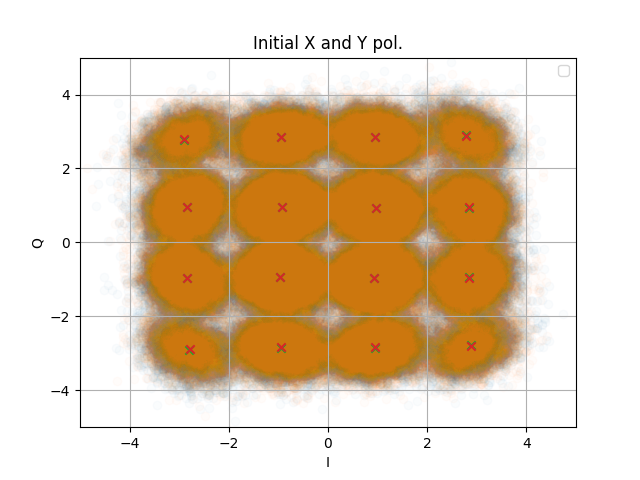
\includegraphics[width=0.48\textwidth]{initial_scatter.png}
}
\subfigure[После фильтрации]{
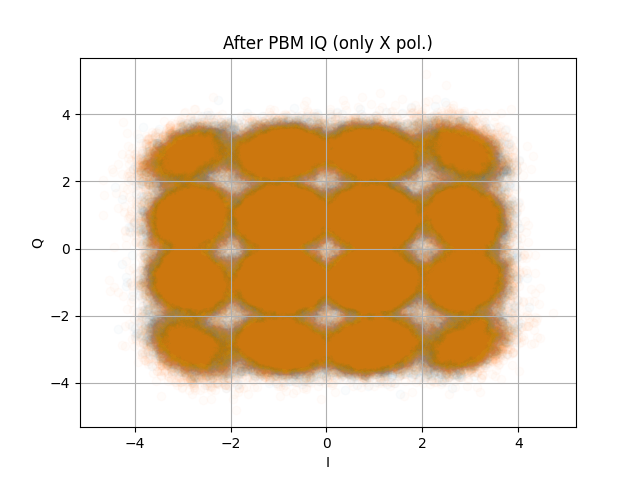
\includegraphics[width=0.48\textwidth]{pbm_scatter.png}
}

\caption{Созвездия}
\label{fig:constel}
\end{figure}

В таблице 1 приведены занчения BER, SER, NMSE и Q для разных значений параметра M.
По таблице построны графики, приведнные на рисунке \ref{fig:perf}.

\begin{table}[H]
    \caption{Производительность PBM}
    \centering
    \begin{tabular}{|l|l|llll|}
    \hline
    \multirow{2}{*}{Метрика} &                                                   & \multicolumn{4}{c|}{M}                                                                          \\ \cline{2-6} 
                             & \begin{tabular}[c]{@{}l@{}}без\\ PBM\end{tabular} & \multicolumn{1}{l|}{3}       & \multicolumn{1}{l|}{5}       & \multicolumn{1}{l|}{10}      & \multicolumn{1}{l|}{15} \\ \hline
    BER                      & 7.47e-3                                           & \multicolumn{1}{l|}{6.01e-3} & \multicolumn{1}{l|}{5.37e-3} & \multicolumn{1}{l|}{4.21e-3} & \multicolumn{1}{l|}{3.38e-3}   \\ \hline
    SER                      & 2.95e-2                                           & \multicolumn{1}{l|}{2.38e-2} & \multicolumn{1}{l|}{2.13e-2} & \multicolumn{1}{l|}{1.67e-2} & \multicolumn{1}{l|}{1.35e-2}   \\ \hline
    NMSE, dB                 & -12.61                                            & \multicolumn{1}{l|}{-12.95}  & \multicolumn{1}{l|}{-13.07}  & \multicolumn{1}{l|}{-13.37}  & \multicolumn{1}{l|}{-13.64}  \\ \hline
\end{tabular}
\end{table}

\begin{figure}[H]
    \centering
    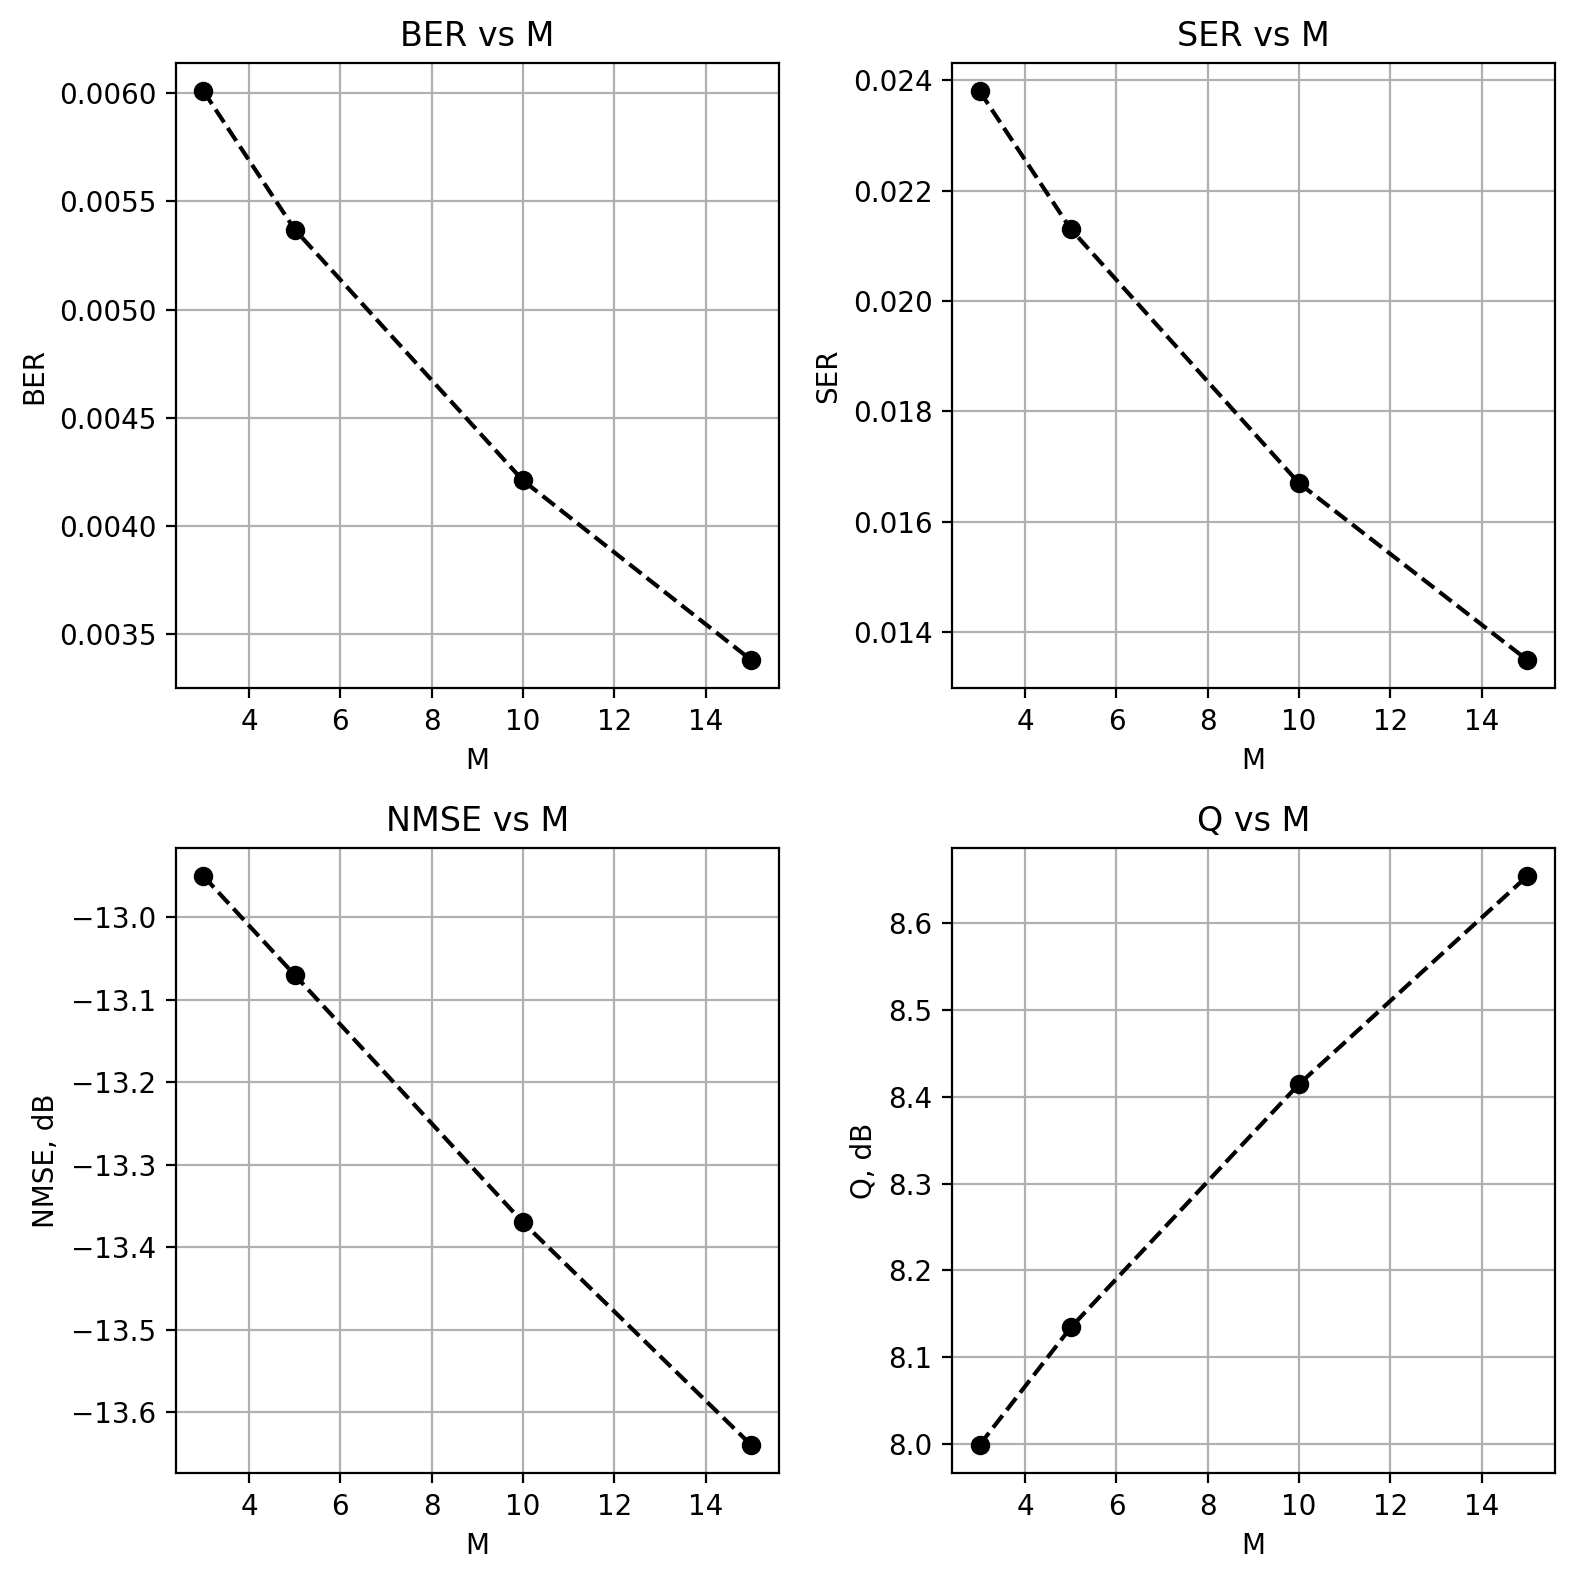
\includegraphics[width=1\textwidth]{performance.png}
    \caption{Влияние параметра M на результат фильтрации}
    \label{fig:perf}
\end{figure}

\end{document}
